\section{GM-6. Singleton}

\subsection*{Problema}
La configuración y el perfil deben consultarse desde diferentes estados sin crear copias con valores divergentes.

\subsection*{Contexto}
La aplicación inicializa LibGDX antes de acceder a las preferencias; el flujo ordinario se ejecuta en el hilo principal.

\subsection*{Solución y aplicación}
\texttt{ConfiguracionJuego} tiene constructor privado, instancia estática privada y acceso mediante \texttt{getInstancia()}. \texttt{GameLluvia.create()} obtiene la instancia. El constructor utiliza \texttt{Gdx.app.getPreferences()} y crea el perfil asociado. No es una implementación sincronizada para uso concurrente ni un gestor global de todos los recursos.

\subsection*{Evidencia}
\begin{itemize}
\item \href{https://github.com/maverick1006/Proyecto-Game-LLuvia-/blob/entrega-final/core/src/main/java/puppy/code/ConfiguracionJuego.java#L7}{ConfiguracionJuego.java, línea 7} (\texttt{private static ConfiguracionJuego})
\item \href{https://github.com/maverick1006/Proyecto-Game-LLuvia-/blob/entrega-final/core/src/main/java/puppy/code/ConfiguracionJuego.java#L13}{ConfiguracionJuego.java, línea 13} (\texttt{private ConfiguracionJuego()})
\item \href{https://github.com/maverick1006/Proyecto-Game-LLuvia-/blob/entrega-final/core/src/main/java/puppy/code/ConfiguracionJuego.java#L19}{ConfiguracionJuego.java, línea 19} (\texttt{public static ConfiguracionJuego getInstancia()})
\item \href{https://github.com/maverick1006/Proyecto-Game-LLuvia-/blob/entrega-final/core/src/main/java/puppy/code/GameLluvia.java#L37}{GameLluvia.java, línea 37} (\texttt{configuracion = ConfiguracionJuego.getInstancia()})
\end{itemize}

\clearpage
\begin{figure}[p]
\centering
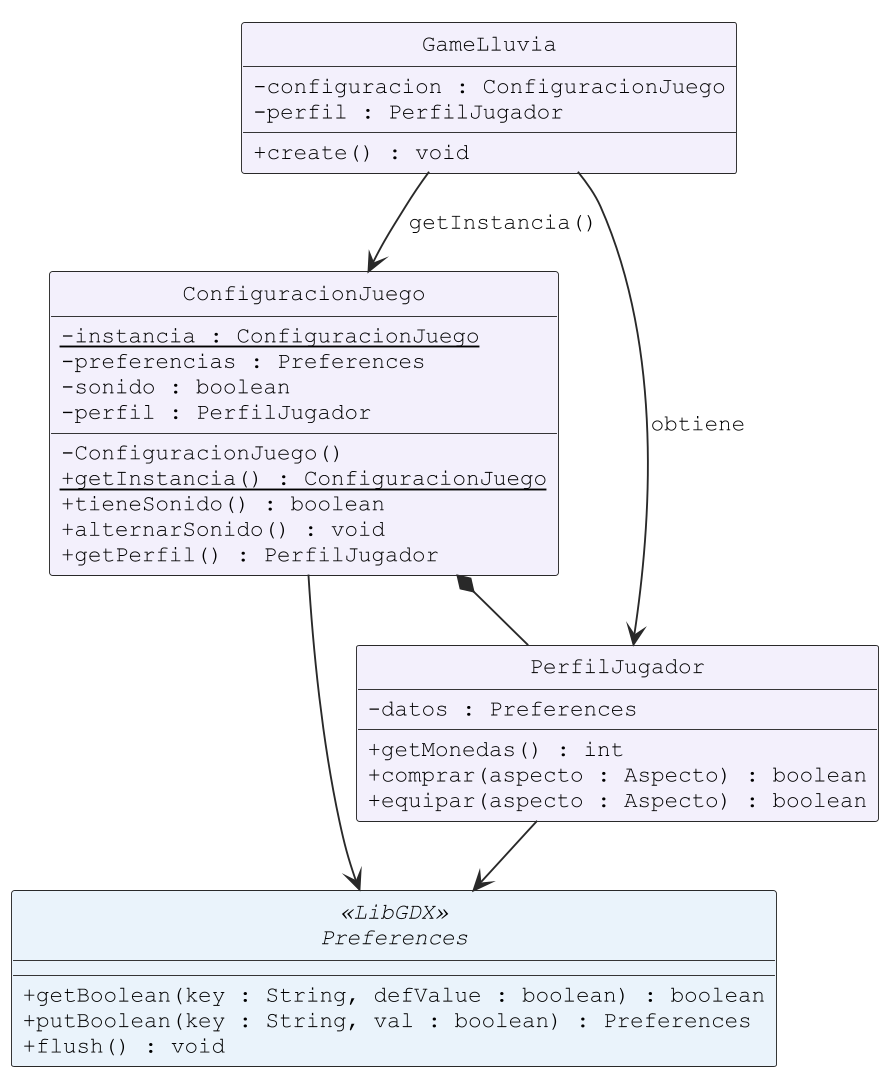
\includegraphics[width=0.95\linewidth,height=0.84\textheight,keepaspectratio]{images/02-singleton.png}
\caption{Singleton de configuración y acceso al perfil}
\end{figure}




